% !TeX root = ../dissertation.tex

\section{Implementing representatives of each virtualization scheme}
\label{representative}

Existing GPU virtualization solutions~\cite{dowty2009gpu, VGML} support
graphics frameworks like Direct3D~\cite{directX}, OpenGL~\cite{openGLspec}.
In principle, there should be no fundamental difference between GPU
virtualization for graphics versus \emph{compute} workloads: ``compute
shaders'' are implemented by the hardware as an additional stage in the
graphics pipeline~\cite{gpu_shader}. In practice, they have significantly
different goals: For graphics, virtualization designs target an interactive
frame rate (18-30 fps~\cite{frame_rate}). For GPGPU compute, virtualization
designs must preserve the raw speedup achieved by the hand-optimized GPGPU
application, which is a considerably harder target to hit. As a result, GPGPU
virtualization remains an open problem. While graphics devices have long
enjoyed well-defined OS abstractions and interfaces~\cite{winGDI}, research
attention to OS abstractions for GPGPUs~\cite{rossbach2011ptask, dandelion,
silberstein2013gpufs, timegraph, gdev, gpunet} has yielded little consensus.
This section describes each of the systems that we chose to represent each of
the canonical virtualization schemes in our empirical analysis, and how we modified or implemented them.

\subsection{GPUvm}
As a representative of full and para-virtual schemes, we chose to study
GPUvm~\cite{suzuki2014gpuvm}, a Xen-based virtualization scheme for NVIDIA's
Kepler and Fermi GPUs. A simplified block-diagram representation is shown in
Figure~\ref{fig_gpuvm_basic}). GPUvm presents each VM with a GPU device model,
which is emulated in the privileged domain (Dom 0). Attempts to access the GPU
from all VMs are interposed via traps and are routed through a GPU Aggregator.
The  aggregator maintains shadow page tables, shadow channels, implements a
``fair share scheduler'', and modifies requests to enforce isolation. GPUvm
interposes on communication between guest device driver and the GPU device
model, by trapping and forwarding MMIO writes. The authors also explore a
number of optimizations: lazy shadowing, bar remap, para-virtualization, and
multi-call batching. GPUvm has not been maintained: The last release, in 2012,
is based on Xen 4.2.0 and runs on Fedora~16~\cite{yu2017fullvirt}. In order to
compare all of the representatives on the same modern platform, we ported
GPUvm to Ubuntu~16.04 with Xen~4.8.2.

\begin{figure}[!th]
	\centering
	\begin{subfigure}{.45\columnwidth}
		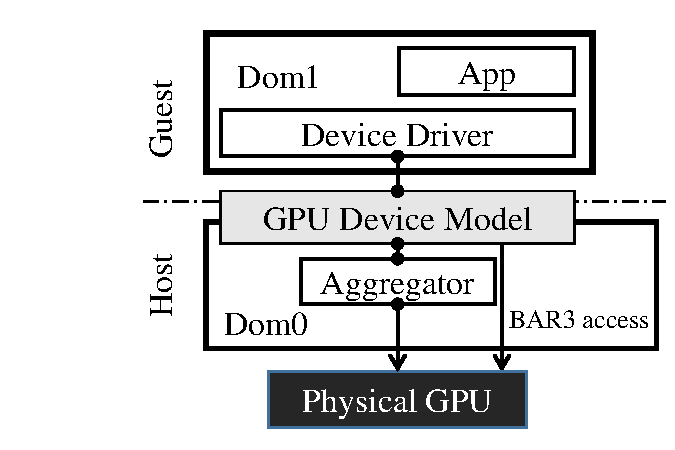
\includegraphics[width=\columnwidth,trim={2cm 0cm 0cm 0cm},clip]{trillium/images/design/gpuvm.pdf}
		\caption{{}}
		\label{fig_gpuvm_basic}
	\end{subfigure}\hfill
	\begin{subfigure}{.55\columnwidth}
		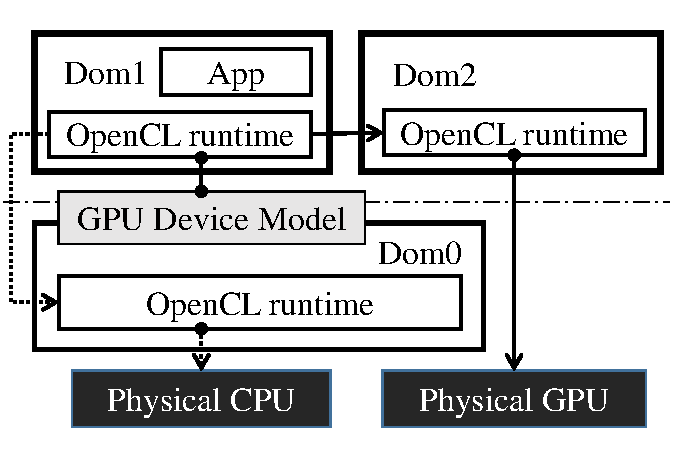
\includegraphics[width=\columnwidth,trim={0 0 0 0},clip]{trillium/images/design/api-remote.pdf}
		\caption{{}}
		\label{fig:api_remote}
	\end{subfigure}
	\caption{{\footnotesize Xen-based virtualizaton designs. (a) GPUvm. (b) User-space API remoting over RPC---dashed arrows indicate \apicpu, while solid ones indicate \apigpu.}}
\end{figure}

\subsection{User-space API remoting}

In order to faithfully mimic user-space API-remoting systems~\cite{rCUDA,
kim2012snucl,bitfusion-whitepaper}, we implemented a system on Xen that trapped
OpenCL API calls using a user-space shim library. These trapped calls were
then forwarded, via RPC, from one appliance VM (the ``client'') to another
appliance VM (the ``server''). Figure~\ref{fig:api_remote} shows the setup of
the two API-remoting schemes we considered: \apigpu and \apicpu.
The black arrows indicate the workflow of \apigpu, where the OpenCL server
ran the OpenCL commands on a physical GPU using the NVIDIA OpenCL framework.
The grey arrows show the \apicpu setup, where the OpenCL commands were
executed on a multi-core CPU (Intel CPU Xeon E5-2643) using the Intel OpenCL
SRB~5.0 framework. The remoting itself was accomplished using gRPC~1.6
(ProtocolBuffers~3.4.0) and inter-service communications were implemented over
XML-RPC~1.39. Lower-overhead data-movement techniques, such as zero-copy, can
be applied when both the client and the server are on a local machine, but
were not considered in our implementations.


\begin{figure*}[!th]
	\centering
	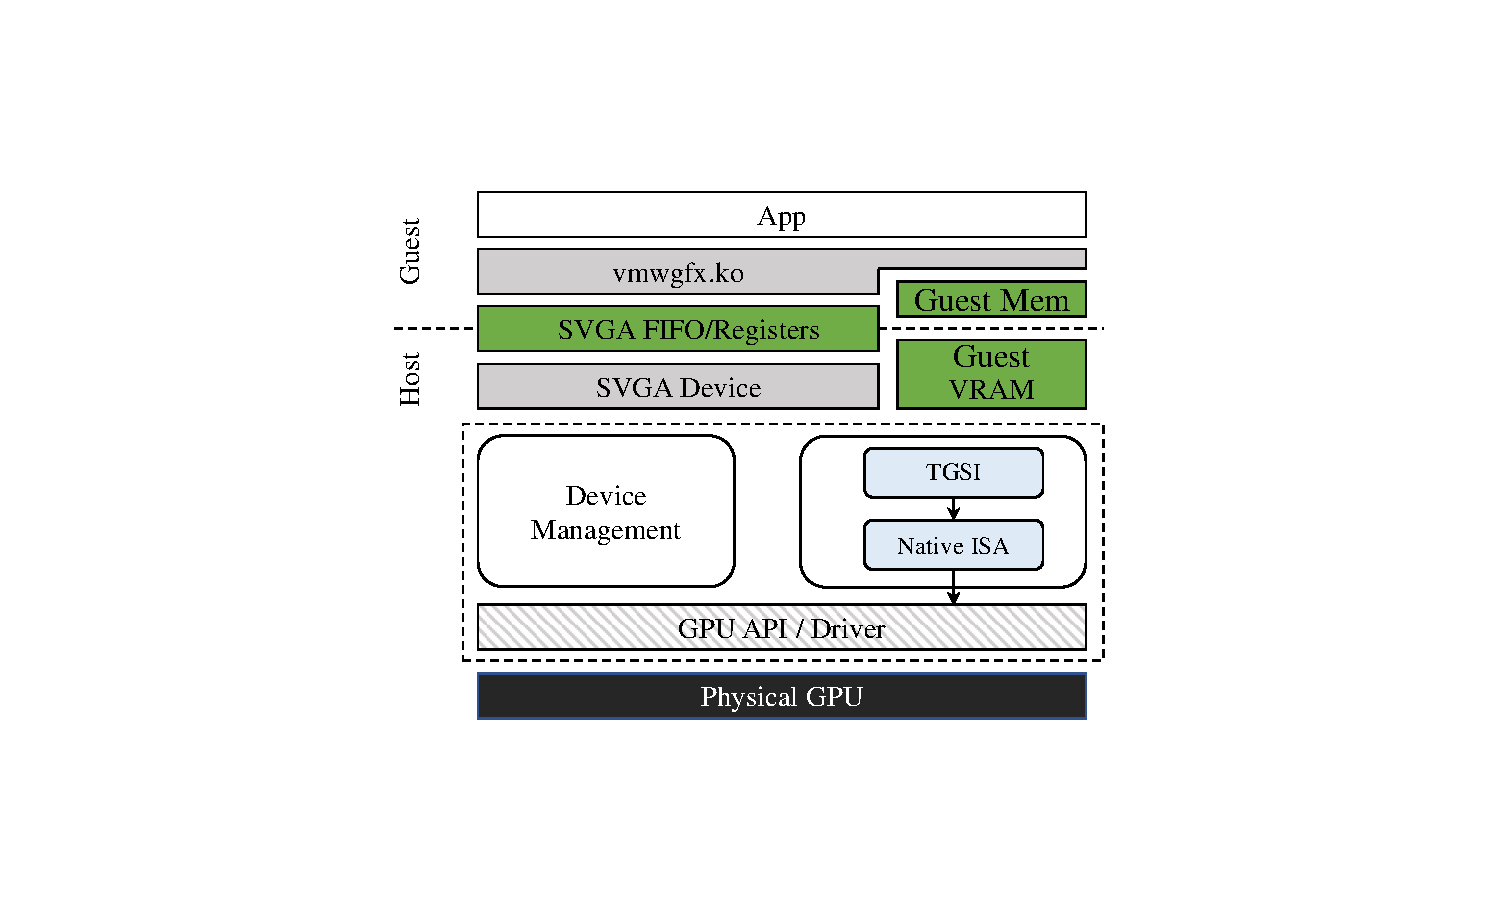
\includegraphics[width=.5\linewidth,trim={6cm 3cm 6cm 3cm},clip]{trillium/images/svga.pdf}
	\caption{{\footnotesize Stack diagram of the SVGA virtualization scheme.}}
	\label{fig_svga}
\end{figure*}

\subsection{SVGA}

SVGA~\cite{dowty2009gpu} remotes DirectX and OpenGL over an emulated (
software) PCIe device. The SVGA virtual device behaves like a physical GPU, by
exporting virtual resources in the form of registers, extents of guest memory
accessible to the virtual device, and a command queue. I/O registers (used for
mode switching, IRQs, memory allocation) are mapped in an interposed PCIe Base
Address Register (BAR) to enable synchronous emulation. Access to GPU memory
is supported through asynchronous DMA. Figure~\ref{fig_svga} presents an
overview of SVGA.

SVGA combines many aspects of full-, para-virtual and API remoting designs.
Unmodified guests can transparently use SVGA as a VGA device, making full
virtualization possible where necessary. However, access to GPU acceleration
requires para-virtualization through VMware's guest driver. As in a physical
GPU, SVGA processes commands from a memory mapped command queue; unlike in a
physical GPU, the command queue functions as a transport layer for APIs
between the guest graphics stack and the hypervisor.

SVGA uses the DirectX~\cite{directX} API as its internal protocol, thereby
realizing an API-remoting design. The transport layer and protocol are
completely under the control of the hypervisor, enabling many of the benefits
of API-remoting while ameliorating its downsides. However, using the DirectX
API as a transport protocol requires that the driver and hypervisor translate
guest interactions into DirectX whether they are natively expressed in DirectX
or not. Coupling the transport layer with a particular version of the DirectX
protocol has led to serious complexity and compatibility \textit{challenges}:
supporting each new version of the API takes many person-years (VMware
introduced support for DirectX 10 (released in 2006) in 2015!).

SVGA also relies on a virtual GPU ISA called TGSI~\cite{tgsi}. TGSI maps
naturally to the graphics features of the ISAs it was originally designed to
encapsulate, but has failed to keep up with GPU ISAs that have evolved to
support general purpose computation primitives. Further, mapping TGSI to all
possible physical GPU ISAs is a herculean task that was doomed from the outset.

\begin{figure*}[!th]
	\centering
	\begin{subfigure}{.5\linewidth}
		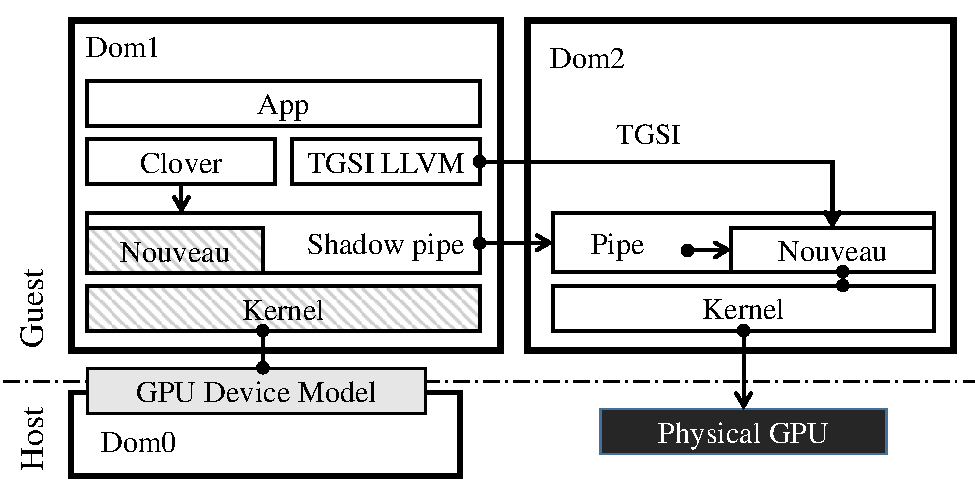
\includegraphics[width=\columnwidth,trim={0 0 0 0},clip]{trillium/images/design/xen-svga.pdf}
		\caption{{}}
		\label{fig_trillium_classic}
	\end{subfigure}\hfill
	\begin{subfigure}{.5\linewidth}
		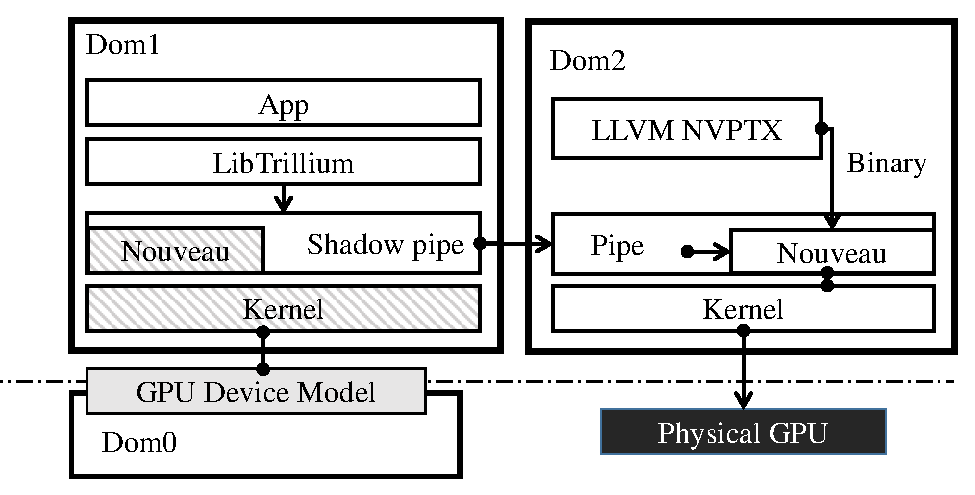
\includegraphics[width=\columnwidth,trim={0.6cm 0 0 0},clip]{trillium/images/design/trillium.pdf}
		\caption{{}}
		\label{fig_trillium_direct}
	\end{subfigure}
	\caption{{\footnotesize \XenSVGA and \Trillium designs. (a) \XenSVGA approximates the SVGA model extended to support GPU Compute. (c) The design of \Trillium with shadow pipe.}}
\end{figure*}

\subsection{\XenSVGA and \Trillium}

We initially implemented the SVGA~\cite{dowty2009gpu} model on Xen strictly
keeping with the original design: we implemented OpenCL support in a virtual
device and extended the Mesa stack with TGSI support (see Section~\ref{ssec:tgsi_backend} for details). The generated TGSI is sent to the host via
RPC, and then finalized to a binary that can be run on the physical NVIDIA GPU
using the open source Nouveau driver. This faithful implementation, hereafter
called \XenSVGA, is used in our study as a representative of the original SVGA
design. \XenSVGA is shown in Figure~\ref{fig_trillium_classic}.

In order to test our hypothesis about vISAs, we modified \XenSVGA to elide the
TGSI compiler, thus arriving at \Trillium. \Trillium forwards API calls for
compiling OpenCL code to the hypervisor. The OpenCL compiler in the host
OpenCL framework (optimized for the physical hardware by the hardware vendor)
is invoked on the forwarded OpenCL code to lower it directly to the physical
device ISA. Figure~\ref{fig_trillium_direct} shows the Trillium design in the
Xen hypervisor stack. The OpenCL API is forwarded from the driver similar to
\XenSVGA. The OpenCL compute kernel (to be run on the GPU) is passed through to
the host via hypercalls in the driver, without being translated to TGSI, where
it will be translated and optimized for the physical GPU in a virtual
appliance (Dom~2 in Figure~\ref{fig_trillium_direct}).

\XenSVGA and \Trillium export an abstract virtual device and a para-virtual
guest driver, which we use to interpose and forward the OpenCL and CUDA APIs
to the host. Unlike SVGA, which requires translation layers to ensure that all
graphics frameworks APIs can be mapped to the SVGA protocol, \XenSVGA and
\Trillium forward the lowest layer in the GNU/Linux Graphics stack: the
pipe-driver, effectively remoting OpenCL/CUDA API calls in the guest to the
OpenCL/CUDA library in the host.

\XenSVGA and \Trillium, implement API-forwarding in a custom pipe-driver in
Gallium3D, that we call \shadowpipe. We chose to forward the pipe-driver as it
is presents a narrow interposition interface in the graphics driver. However,
given that each OpenCL API call is decomposed into many different pipe-driver
calls, other APIs higher up in the graphics stack may be better suited for
interposition. The \shadowpipe is in the \textit{application domain}'s graphics
stack, and shims the pipe-driver interface as RPC calls to the actual Nouveau
pipe-driver in the \textit{privileged domain}.

\XenSVGA and \Trillium manage user-level contexts, command queues and memory
objects. While \XenSVGA relies on our TGSI compiler to translate the input
OpenCL GPGPU kernel to TGSI in the application domain, \Trillium skips the
compilation phase. Instead, the OpenCL kernel is forwarded to the privileged
domain via RPC, where it is parsed and compiled by the LLVM NVPTX back-end in
parallel. This binary is then loaded onto the GPU when the pipe-driver hits
the binary loading phase. \Trillium can also emit LLVM IR if an OpenCL
compiler is not available in the host.

Our implementation relies on gRPC as a transport mechanism between the guest
and the host, as an implementation convenience. As zero-copy transfer~\cite{
chu1996zero,tezuka1998pin} and hypercall~\cite{ram2010redesigning} mechanisms
are well-studied, and a production-ready version of \Trillium would rely on
these mechanisms, we measure and remove transport overhead from our reported
measurements in Section~\ref{sec:trilliumeval}.
The overheads stem from remoting calls to the privileged domain over the
network, which is especially significant since a single OpenCL API call may be
decomposed into many pipe-driver APIs, and from the large amount of kernel
input data that must be copied between VMs.
\XenSVGA and \Trillium do not currently guarantee performance isolation,
although this can easily be implemented via a rate-limiting API scheduler in
the hypervisor, as in GPUvm~\cite{GPUvm}.

\subsubsection{Mesa3D OpenCL Support}

The Mesa3D Graphics Library~\cite{mesa} is an open-source graphics framework
that implements graphics runtime libraries (e.g., OpenGL~\cite{openGLspec},
Vulkan~\cite{Vulkanspec}, Direct3D~\cite{directX}, and OpenCL~\cite{
stone2010opencl}) on most GNU/Linux installations. It also includes official
device drivers, written in a common framework, Gallium3D~\cite{gallium}, for
Intel and AMD GPUs. Support for NVIDIA GPUs is provided via reverse-engineered
open-source driver, Nouveau. Gallium3D imposes TGSI as the common virtual ISA
for compute shaders, and decomposes drivers into two components: \textit{state
trackers}, which keep track of the device state, and \textit{pipe drivers},
which provide an interface for controlling the GPU's graphics pipeline (e.g.
translate the state, shaders, and primitives into something that the hardware
understands). Effort is underway to replace TGSI with SPIR-V and LLVM IR, but
it wasn't mature when we undertook this project.

OpenCL support was first introduced in Mesa3D 9.0 with the release of the
Clover state tracker. Clover supports OpenCL~1.1 and was mainly contributed by
AMD developers. It was envisioned that Clover would leverage the LLVM~\cite{
lattner2004llvm} compiler to lower the OpenCL source to TGSI. Despite much
effort by the open-source community~\cite{old_llvm_tgsi1,old_llvm_tgsi2}, an
LLVM TGSI back-end has remained incomplete. Clover currently supports an
incomplete set of OpenCL~1.1 APIs on AMD GPUs and fails to operate correctly
on NVIDIA GPUs.

\subsubsection{LLVM TGSI Back-end}
\label{ssec:tgsi_backend}
While Clover provides the library for the OpenCL application to link against,
most of the compilation is handled by invoking the OpenCL and C++ front-ends
of the LLVM~\cite{lattner2004llvm} compiler framework. Clover provides much of
the front-end infrastructure required to support GPGPU computing in \XenSVGA
and \Trillium. However, LLVM lacks a working TGSI back-end, which presented a
challenge for \XenSVGA.

In order to support OpenCL in \XenSVGA, we implemented an LLVM TGSI back-end.
While the TGSI back-end is not yet mature, we added support for a majority of
the 32-bit integer and floating point operations, intrinsics, memory barriers,
and control flow. Using this backend we were able to compile and run 10 out of
the 12 Rodinia benchmarks~\cite{che2009rodinia} used to benchmark GPUvm.
Because the compiler was built using the LLVM framework, it enjoyed all of the
IR-level optimizations in LLVM.

LLVM IR handles control flow by using conditional and unconditional branches
to and from Basic Blocks. A majority of the usual optimizations (constant
propagation, loop unrolling, etc) are applied on the IR. On the other hand,
TGSI assumes a linear control flow through the program, using higher level
constructs such as IF-THEN-ELSE, FOR and WHILE loops. To accommodate this
difference in control flow techniques, we leveraged a similar implementation
in the AMDGPU back-end which calculates a Strongly-Connected-Components (SCC)
graph from the Basic Block-based control flow in the LLVM IR, and then
duplicates Basic Blocks as necessary. It is a testament to the maturity and
flexibility of LLVM that the infrastructure to produce an SCC, and an example
of how to use it to raise the control flow abstraction level were readily
available.

\subsection{GPU ISAs and IRs}

IRs are of great interest to the realm of virtualization because an IR that is expressive enough to be able to take advantage of new HW developments, while also being universally accepted by all the competing parties will make a wonderful virtualization primitive.

Intermediate Representations are incredibly useful tools to hardware vendors
as well, enabling them to simultaneously:
\begin{itemize}[nosep, topsep=0em, leftmargin=1em,labelwidth=*,align=left]
\item preserve backward compatibility without compromising innovation at the ISA. The publicly available vISA can be held constant, while the physical ISA is free to change across generations of hardware,
\item have the ability to re-optimize legacy code for new HW without having a dependency on the high level toolkit that generated the code in the first place,
\item have the freedom to optimize their hardware any way they see fit without having to worry about the effect of said optimizations on the ISA,
\item simplify their tool-chain building process by having to only modify one piece---the software that translates from IR to physical ISA) with each new generation of HW,
\item and the ability to leverage open source frameworks like LLVM without having to give up their secret sauce.
\end{itemize}

Given these properties, it comes as no surprise that both AMD and Nvidia both
have a public vISA that is stable across generations (i.e. IL and PTX
respectively), and a physical ISA that is free to evolve with each generation
of hardware (i.e., GCN and SASS respectively). AMD and Nvidia's front-end
compilers generate code in their proprietary vISAs (NVIDIA PTX and LLVM IR for
AMD), and then subsequently finalize this code to the native ISA (SASS and
GCN) using JIT compilers in the GPU driver . The vISA remains stable across
generations to preserve compatibility, while the physical ISA is free to
evolve. TGSI, the virtual ISA used in both the Mesa stack and SVGA, plays a
similar role in the graphics realm---enabling interoperability between graphics frameworks and GPUs from different vendors.

As is often the case in a space where competition is fierce, standardization
is hard to come by.Despite efforts by standards organizations~\cite{Vulkanspec}
to convince competing parties to find a middle ground, so as to give tool
writers some semblance of sanity, no clear standard IR has emerged in the
GPGPU realm. SPIR-V~\footnote{https://www.khronos.org/spir/} is the latest
challenger to walk this gauntlet.

We observe that LLVM IR is in a unique position to become a standard IR.
LLVM has become the de-facto standard for building compilers: both NVIDIA and
AMD use it to implement their virtual ISA compilers, as do all the compilers
in the Mesa stack including the TGSI compiler we implemented. The framework
supports a wide array of front-end languages including CUDA and OpenCL among
others, and a wide array of back-ends as well, including other IRs like SPIR-V.

\subsection{Optimizations}
\label{sec:optimizations}
\Trillium interposes at the pipe-driver API yielding fine-grained
interposition, and therefore fine-grained multiplexing of the GPGPU.
However, interposing at this layer also results in significant transport
overhead. Many pipe-driver functions are responsible for context management
and information retrieval---operations that do not result in interaction with
the GPU. We reduce communication overhead by batching these types of
API-calls, taking care to fall back to synchronous API-forwarding when any
pipe-driver API calls that interact with the physical GPU are invoked.

We optimize the \apigpu and \apicpu systems by preinitializing the device and
preallocating contexts and command queues on the privileged domain. These
contexts are assigned to applications as they execute context creation APIs
and are reclaimed asynchronously.